%! Author = constantinoskavadias
%! Date = 16/10/2022

\documentclass[a4paper,twocolumn,11pt]{quantumarticle}
\pdfoutput=1
\usepackage[utf8]{inputenc}
\usepackage[english]{babel}
\usepackage[T1]{fontenc}
\usepackage[numbers]{natbib}
\usepackage{listings}

\usepackage{amsmath}
\usepackage{amssymb}
\usepackage{hyperref}
\usepackage[resetlabels]{multibib}
\usepackage{graphicx}
\graphicspath{ {./images/} }

\newcites{article}{article references}
\newcites{book}{book references}
\newcites{misc}{misc references}
\newcites{repo}{repository references}
\newcites{web}{website references}
\newcites{other}{Other references}

\begin{document}
    \title{Quantum Natural Language Processing: A look at current applications on NISQ devices}

    \author{Constantinos Kavadias}
    \affiliation{University of Melbourne}
    \email{ckavadias@student.unimelb.edu.au}

    \maketitle
    \begin{abstract}
    In this literature review we will discuss the emerging field of Quantum Natural Language Processing (QNLP), focussing
    in particular on recent developments in small to medium scale experimentation in classification tasks.
    We will discuss and review two experiments one dealing with binary classification tasks in english and the other
    displaying properties of language independence in QNLP circuits for these tasks.
    In order to provide sufficient context to the reader on the concepts that make up the background of these
    experiments the review will also discuss in sufficient detail the DisCoCat\cite{discocat} categorical classification
        for encoding natural language grammar and how this relates to quantum circuits.
    Finally, the review will include a small discussion on an experiment that attempts to replicate the classification
        experiment discussed.
    \end{abstract}

    \section{Introduction}\label{sec:introduction}
    QNLP is the process of applying near term quantum computing techniques to NLP tasks\cite{qnlp_near_term}.
    To understand what this means and the experiments to be discussed in Section~\ref{sec:classification_exp} an understanding
    NLP is necessary.
    NLP is a collection of processes or techniques for analysing the intent or meaning of natural speech and text\cite{nlp},
    achieved with rule based language modelling and artificial intelligence techniques\cite{nlp}.
    \newline
    QNLP signals a shift in computational linguistics, utilising quantum native structures to make the use Noisy
    Intermediate-Scale Quantum (NISQ) devices\cite{qnlp_in_prac}.
    NISQ devices have a relatively low number of available qubits, making them unsuitable for implementation of
    sophisticated error correction techniques, necessitating the use of simple gate structures and using
    the quantum state to encode contextual information\cite{qubits_speak,qnlp_in_prac}.
    \newline
    Building these circuits utilises the DiscCoCat\cite{discocat, qnlp_near_term} grammar
    encoding to translate natural language sentences into tensor calculus.
    DisCoCat stands for categorical compositional distributional semantics\cite{discocat} and describes the syntactic
    and semantic links between words with tensor operations\cite{discocat}.
    Sections~\ref{sec:discocat_circuits} and~\ref{sec:classification_exp} discuss how DisCoCat diagrams can be converted
    to quantum circuitry.
    \newline
    Binary classification has been implemented on NISQ devices\cite{qnlp_in_prac}, classifying both semantic field and
    grammatical differences in sentences\cite{qnlp_in_prac}.
    Extensions of this work have shown that the generated circuits used in these assessments are also language independent\cite{lang_indp}
    with examples from English and Urdu\cite{lang_indp}.
    \newline
    A small scale experiment to perform binary sentiment analysis on a randomised dataset of sentences has been run.
    The sentences are statements generated using a simple context free grammar, following the example of previous QNLP
    experiments\cite{qnlp_in_prac, lang_indp}.
    This experiment provides insights into performance on physical quantum devices and verifies previous findings.

    \section{DisCoCat and Quantum Circuits}\label{sec:discocat_circuits}
    In this section a sufficient explanation of DisCoCat is provided to contextualise the remaining
    sections of this document.
    It will provide insight into what DisCoCat is and hwo it relates to QNLP.
    A commentary is given on assertions made about its suitability in QNLP applications.
    \subsection{What is DisCoCat?}\label{subsec:what-is-discocat}
    Let's recap on what we know about DisCoCat so far.
    DisCoCat is a form of categorical, distributional, compositional grammar\cite{discocat} which means the following:
    \begin{itemize}
        \item It represents different parts of speech as types
        \item Each element of a sentence has a type
        \item Types can be the multiplicative combination of other simple types
        \item The types of all elements of a sentence combine to provide the overall sentence type
        \item Sentence representations can be concatenated to represent equivalent concatenated sentences
    \end{itemize}
    \newline
    In practice DisCoCat describes grammatical types as vectors or matrices which can be assigned to different parts
    of speech\cite{qnlp_in_prac}.
    These types are then connected to each other in operations which can be implemented by tensor products\cite{qnlp_in_prac}.
    Already we start to see how DisCoCat can become an analogue for the vector spaces used in quantum circuits.
    Types start to look like qubits (described by a vector), interactions between one type and another are then naturally
    described by operators acting between wires.
    Figure~\ref{fig:discocat-diagram} provides an example of a DisCoCat diagram which illustrates this wire like property
    of types, note how the word \textbf{hate} is made up of 3 wires representing three simple types.
    \begin{figure}[h]
        \centering
        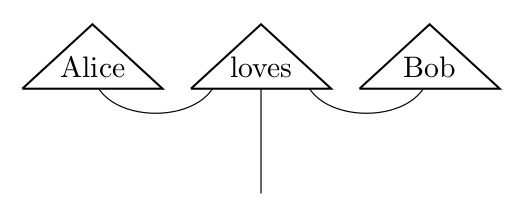
\includegraphics[width=0.25\textwidth]{alicelovesbob}
        \caption{An example DisCoCat diagram for the sentence "Alice loves Bob".}
        \label{fig:discocat-diagram}
    \end{figure}
    Much of the QNLP literature asserts that DisCoCat is a natural analogue to quantum circuits and a sensible
    approach to converting grammar into useful quantum forms\cite{qnlp_in_prac, qnlp_near_term}.
    This assertion relies on the assumptions that DisCoCat provides a good approximation for the Hilbert
    space representation of quantum theory (on which quantum computing relies) and the tensor structures allow for
    multiple orders, making them an analogue for multi qubit operations.
    Both of these assertions essentially imply that DisCoCat can be easily mapped into quantum circuitry, in fact the
    literature even provides an in depth formulation for this conversion\cite{qnlp_near_term} the result of which is shown in
    Figure~\ref{fig:quantum-circuit}.
    \begin{figure}[h]
        \centering
        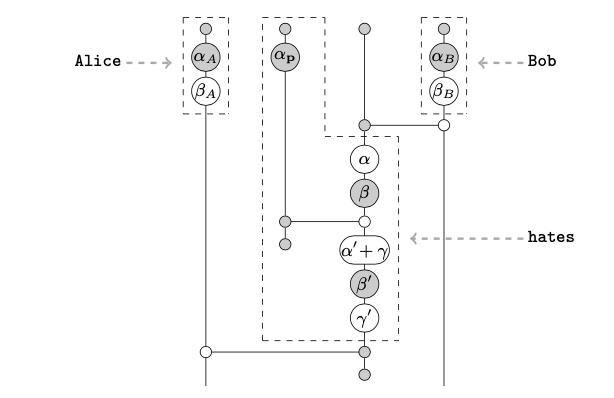
\includegraphics[width=0.5\textwidth]{quantum-circuit}
        \caption{An example quantum circuit for the sentence "Alice hates Bob"\cite{qubits_speak}.}
        \label{fig:quantum-circuit}
    \end{figure}
    Do these assertions add up?
    Are they reasonable?
    For the reasons provided in the literature the answer appears to be yes.
    The Hilbert space formulation of quantum theory is a multi-dimensional tensor
    space, by definition the same is true of DisCoCat\cite{discocat}.
    The circuit mapping process provided is also rigorous\cite{qnlp_near_term} with each step sourced and explained in
    such a way that the reader can easily replicate it, this will be further shown by the novel experiment at the end
    of this paper.
    The assertion that DisCoCat provides an analogue for quantum circuitry appears well defended and well considered.
    \subsection{From speech to circuits}\label{subsec:from-speech-to-circuits}
    Classical NLP uses machine learning techniques to interpret patterns in natural language and discern meaning.
    These techniques are, unfortunately, not feasible on available quantum computers, they require advance I/O
    operations and access to RAM that cannot be achieved by NISQ devices\cite{qubits_speak}.
    Given these limitations an alternative is the direct mapping of sentences (syntactically and semantically) into quantum
    circuits\cite{qubits_speak, qnlp_in_prac}, using the DisCoCat representation of grammar.
    This process can be described as follows for a known corpus\cite{qnlp_near_term}:
    \begin{enumerate}
        \item Define a pregroup grammar\cite{qnlp_near_term} for the corpus
        \item Covert the grammar into DisCoCat grammar diagrams
        \item Perform a diagram simplification\cite{qnlp_near_term}
        \item Select an ansatz for each POS and associated parameters for each lexeme in the grammar
        \item Replace elements of the DisCoCat diagrams with ansatz gates
    \end{enumerate}
    The result of this process is a programmable quantum circuit.
    This is a method for building syntactic circuits from sentences.
    To insert the required semantic context they are treated as variational quantum circuits, optimisation is
    performed to learn the necessary parameters of the ansatz\cite{qubits_speak}.
    With the parameters known circuits can be built to represent novel sentences formed from the known grammar and lexemes.
    \newline
    This method only supports context free grammars using known lexemes\cite{qubits_speak} and is incapable
    of describing the full extent of natural language.
    However, it provides a testable, reusable and deterministic framework for building
    quantum circuits to represent simple language.
    While not suitable for more advanced NLP on contextual grammars it is promising
    and shows that current limitations are not a blocker for development in this space.
    The authors acknowledge the limitations and the possibility of extension.
    Varying grammatical models can be encoded in DisCoCat\cite{qnlp_in_prac}.
    These include verb modelling and word relations like homonymy using density matrices.
    With these extensions the method is promising especially on NISQ devices.
    Using ansatz and variational quantum circuitry to encode complex information allows the practical
    application of theoretical work that would otherwise be blocked by quantum device limitations.
    \section{Classification Experiment}\label{sec:classification_exp}
    In this section we will look at a classification experiment using the described QNLP circuit building.
    The experiment includes two corpora and shows an pplication of binary classification using this method.
    \subsection{The experiment}\label{subsec:binary-classification}
    Binary classification is a NLP task involving classifying sentences as belonging to one of two categories.
    In this experiment two different corpora were used, the first is topic based containing sentences
    about IT or food\cite{qnlp_in_prac}, the second is grammatical with sentences containing an object or
    subject based relative clause.
    Both experiments used the DisCoCat method for circuit construction and learning word  parameterisations for the circuits.
    The use of DisCoCat in these scenarios was interesting as it showed how the model can be manipulated to change
    what is considered grammatical to suit different goals and corpora\cite{qnlp_in_prac}.
    \newline
    Variational training phases were performed using classical simulations of quantum devices.
    This allowed the testing of different ansatz to find the configuration with the lowest training cost function
    convergence value without needing an available NISQ device\cite{qnlp_in_prac}.
    This provides confidence in the suitability of the chosen ansatz.
    During the physical device training phase the winning ansatz from the classical simulations was chosen and the circuits
    constructed with it.
    The authors for reasons of cost and accuracy chose to load the circuits of all sentences in the training corpus as
    a single circuit, the advantages of this approach meant a single optimisation run for all parameters, reducing total
    number of circuit runs on physical devices.
    \subsection{Evaluation}\label{subsec:evaluation}
    Both experiments had promising F-scores when run on test data of 0.85 for the topic classification and 0.75 for
    the syntax classification\cite{qnlp_in_prac}.
    These scores were compared against random guessing and were found to be statistically significant\cite{qnlp_in_prac}.
    The results of these experiments are promising, showing non-trivial success for the classification task.
    They were unable to be accurately compared to a classical counterpart or even a classical simulation of the same
    quantum task due to hardware limitations on number of runs.
    This is disappointing since the error rates of both experiments appeared to be lower on physical hardware compared
    to the simulations but the results are inconclusive\cite{qnlp_in_prac}.
    \subsection{Discussion}\label{subsec:discussion}
    The use of two different classification tasks shows that the efficacy of QNLP classification is not limited to a
    particular domain or grammar and removes potential inclinations towards dataset bias.
    The topic classification task used an artificial corpus constructed for the experiment,
    however the syntax classification task used a filtered set from an existing corpus RELPRON\cite{qnlp_in_prac}.
    This provides confidence that the authors have not used a purpose built corpus to manipulate their results.
    The constructed corpus for the topic classification contained lexemes shared between both domains making the
    sentences non-trivial to classify, this increases our confidence in the efficacy of the method.
    \newline
    If possible it would have been interesting to see a comparison to an equivalent classical task on the same corpus
    rather than a comparison with a classical simulation of the quantum task.
    Given that the author's intention was to simply prove that the QNLP method was practical and useful however its
    absence is not surprising.
    \section{Novel Experiment}\label{sec:novel_exp}
    The novel experiment uses a simple corpus described by the context free grammar in Table~\ref{tab:cfg}
    for sentiment analysis.
    \begin{table}[h!]
        \centering
        \begin{tabular}{|| c ||}
            \hline
            noun phrase → noun \\
            noun phrase → adjective noun \\
            verb phrase → verb noun phrase \\
            sentence → noun phrase verb phrase \\
            \hline
        \end{tabular}
        \caption{Simple context free grammar for test corpus of novel experiment as seen in\cite{qnlp_in_prac}}
        \label{tab:cfg}
    \end{table}
    The main aim of this experiment is to determine whether the results in the previously discussed classification
    experiments are reproducible, for that reason the experiment will have the following features:
    \begin{itemize}
        \item The same ansatz as the topic experiment in Section~\ref{sec:classification_exp}
        \item The same diagram simplification as the topic experiment in Section~\ref{sec:classification_exp}
        \item The same corpus size (65 sentences per sentiment) as the topic experiment in Section~\ref{sec:classification_exp}
        \item The same optimisation function as the topic experiment in Section~\ref{sec:classification_exp}
    \end{itemize}
    The python code running the experiment has been based on an existing QNLP python library\cite{python-lib}
    \subsection{Results}\label{subsec:novel-results}
    Training runs for the experiment were performed using the IBM AER simulator.
    This was due to time constraints, allowing training to be completed without waiting for physical machines to become
    available.
    \newline
    We can see from Figure~\ref{fig:experiment-training} that convergence in training happened around the 100--200 iteration
    mark and that accuracy in both the training and development sets stayed around 0.5 for all iterations with variation
    between 0.54 and 0.46 approximately.
    The convergence and accuracy results of the novel experiment closely match the original topic classification
    experiment\cite{qnlp_in_prac}.
    This provides reassurance that the results in that experiment can be trusted and are reproducible for different
    corpora.
    \newline
    An evaluation run was performed on the IBM physical quantum device \textbf{ibm-oslo} with a resulting accuracy
    on the test corpus of 0.5, this was better than the same evaluation performed on the simulator which scored 0.483.
    While this comparison provides little value in assessing the original experiment it was interesting to note the
    significant accuracy difference.
    The full Jupyter notebook and corpora used for the experiment is available in a public github repository\cite{novel-exp-repo}.
    \begin{figure}[h]
        \centering
        \includegraphics[width=0.5\textwidth]{experiment-training}
        \caption{Training and development set loss and accuracy by iteration\cite{novel-exp-repo}.}
        \label{fig:experiment-training}
    \end{figure}
    \section{Conclusion}\label{sec:conclusion}
    We have seen a discussion about the current state of QNLP and experiments that provide practical insights into that
    state.
    This includes a method for mapping natural language into deterministic quantum circuits and encoding word meaning
    into circuit parameters using variational training methods.
    A discussion of two binary classification experiments was provided ultimately concluding that they show the
    practical application of the new QNLP techniques is promising and extensible but further analysis was limited
    by hardware limitations and accessibility.
    A novel experiment was presented that replicated the binary classification results, using a unique corpus and the same
    ansatz and circuit mapping presented in the original experiment.
    \bibliographystyle{quantum}
    \bibliography{research_project}
\end{document}